%%%%%%%%%%%%%%%%%%%%%%%%%%%%%%%%%%%%%%%%%%%%%%%%%%%%%%%%%%%%%%%%%%%%%%%%%%%%%%
%%
%% This file is part of the ASTERICS Framework. 
%%
%% Copyright (C) Hochschule Augsburg, University of Applied Sciences
%% Efficient Embedded Systems Group
%%
%% Author(s): Gundolf Kiefer <gundolf.kiefer@hs-augsburg.de>
%%
%%%%%%%%%%%%%%%%%%%%%%%%%%%%%%%%%%%%%%%%%%%%%%%%%%%%%%%%%%%%%%%%%%%%%%%%%%%%%%



%%%%%%%%%%%%%%%%%%% 1. Overview %%%%%%%%%%%%%%%%%%%


\chapter{Overview}\label{ch:01-overview}

\secauthor{Gundolf Kiefer, Michael Schäferling, Alexander Zöllner}

\section{Background}

%[[ TBD (AZ/MS/GK) ]]

As FPGAs are growing in their capacities, hardware structures of increasing complexity can be implemented.
This allows to map more sophisticated algorithms to these structures, enabling ever more complex applications.
Due to the wide range of algorithms and their varying requirements on resources and architecture, utilizing heterogeneous platforms is becoming increasingly popular.
These allow to utilize powerful hardware/software codesigns, by utilizing dedicated hardware structures along with a complex software stack, as well as a full-featured operating system.
Modern systems-on-chips (SoCs) even allow to integrate these codesigns on a single chip.

Computer Vision (CV) has been a significant area of research for quite some time and has already benefited various fields of industry, such as detecting faulty parts built by automatized production lines. 
Advances in technology within recent years also enabled using CV for embedded applications, such as advanced driver assistance systems, which use CV for line and traffic sign recognition. 
These tasks are also indispensable for autonomously driven cars.
Another application is validating the status of a construction site's progress, such as determining the number and location of pipework installation within ship and plant constructions.
Here, CV is used for tasks such as detecting geometric primitives and translating them to the actual objects for a CAD model.

However, CV is still a computational and resource demanding task, which is expected to no longer be automatically solved by more powerful processors becoming available due to reaching technological limits in foreseeable future.
Rather, innovative and efficient structures have to be developed to further advance the fields of application using CV.
The \asterics framework already offers dedicated hardware structures for speeding up CV tasks by simultaneously using only little resources. 
Exemplary structures include an implementation of a Hough Transform variant for detecting arbitrary objects and lines~\cite{kiefer_configurable_2016} and a pipeline-based architecture for applying 2D window filters on images~\cite{pohl_efficient_2014}, with more hardware structures being continuously added.

In order to seamlessly integrate \asterics into CV applications and reducing development time, a full-featured software stack is also provided, which can be integrated into an operating system.
Further, integration into the Robot Operating System (ROS) is offered and integration into the commonly used OpenCV library is actively being worked on.

The main goal of \asterics is speeding up and enhancing CV applications in a convenient and efficient manner by utilizing its hardware structures along with its software stack.



\section{What is \asterics}

\subsection{Overview}
\asterics is an open toolbox for building hardware accelerated image processing chains~\cite{EES_ew_2015_asterics}.
Therefor, hardware designs for an increasing range of algorithms are offered, which are developed in the form of self-contained modules.
This allows to combine them to arbitrary image processing chains in a modular manner, in order to meet the requirements of a certain application.
\asterics also contains a number of software drivers and utilities for interfacing its hardware modules.
In order to cover a wide range tasks, \asterics covers all categories for image processing, namely \textit{point operations}, \textit{window filter operations}, \textit{semi-global/patch-based operations} and \textit{global operations}~\cite{pohl_efficient_2014}.
Figure~\ref{fig:01-asterics-example} shows an exemplary image processing chain, where critical aspects of the image processing task is sped-up in hardware.
The results are passed to software using main memory for further processing or may be displayed on a monitor.

%TBD: Hier erst Bild zum kompletten Stack (vgl. ASAP-Paper/-Vortrag) bringen?

\begin{figure}[ht]
    \noindent \begin{centering}
        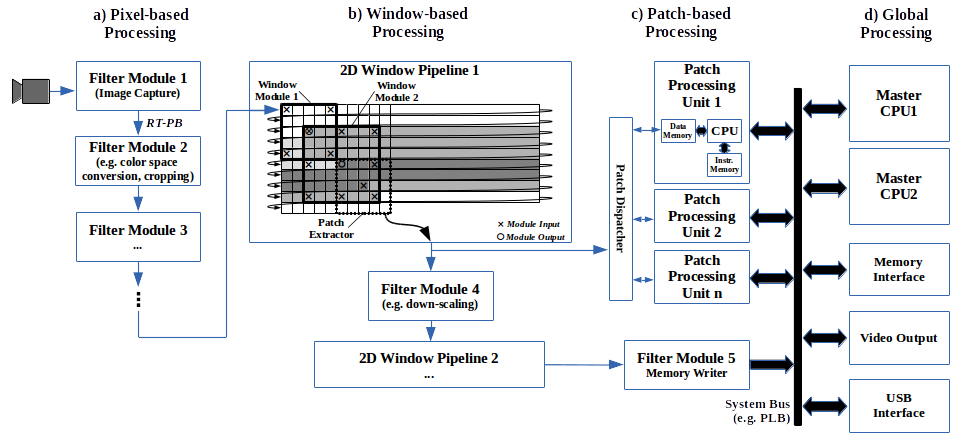
\includegraphics[width=15cm]{figs/01-asterics-example}
        \par\end{centering}
    \caption{Example \asterics system\label{fig:01-asterics-example}}
\end{figure}


\subsection{Interfaces}
\asterics utilizes a modular principle for combining its modules to arbitrary image processing chains.
Great effort has been made to create a set of interfaces for defining the inter-module communication and hardware-software interaction to guarantee a certain behavior within the processing chain and to prevent data loss. 
The interfaces of \asterics are organized as following:

\begin{itemize}
    \item General Interfaces (Chapter~\ref{ch:05-01-interfaces-general})
    \item Common Per-Module Signals (Chapter~\ref{ch:05-02-interfaces-module_signals})
    \item The \asterics Streaming Interface (\texttt{as\_stream}) (Chapter~\ref{ch:05-03-interfaces-as_stream})
    \item The \asterics 2D Window Filter Interface (Chapter~\ref{ch:05-03-interfaces-as_window})
\end{itemize}

\subsubsection{General Interfaces}
This type of interfaces covers general concepts for interaction between hardware and software for a single module as well as a processing chain as whole.
Here, the software is accessing the hardware for obtaining status information and influencing the behavior of the hardware.
This includes the types of errors which may occur within the hardware which have to be addressed by software and the expected behavior of the hardware in case the software \textit{resets} single modules or the processing chain as a whole.
Additional topics are the version management and the i2c bus interface for communicating with external hardware components, which are not part of the programmable logic.

\subsubsection{The Common Per-Module Signals}
These interfaces are used for hardware internal communication to request status information and trigger certain operations, which affect modules as a whole.
These status information include the \texttt{READY} signal, which indicates whether the hardware module is currently operable or the \texttt{SYNC\_ERROR} which signals that data has been lost at some point during operation.
Regarding the operations affecting modules as a whole, signals such as \texttt{RESET} and \texttt{FLUSH} may be present for the module.

The aforementioned interfaces can either be utilized by other \asterics hardware module or by some logic for controlling the entire image processing chain, e.g. to reset all modules at once.  

\subsubsection{The \asterics Streaming Interface (\texttt{as\_stream})}
Signals which are required for controlling the actual data transfers between hardware modules, e.g. the inter-module communication, are summarized here.
The signals \texttt{DATA} and \texttt{STROBE} are used for setting up the most basic data transfers.
The \texttt{as\_stream} interface defines additional signals, mainly for synchronization to provide more detailed information about the data layout, e.g. \texttt{HSYNC} for indicating the start of a new line.
Additionally, the \texttt{STALL} signal is defined by the \texttt{as\_stream} interface for requesting to temporarily suspend data transfers, in case data is processed at a varying pace across hardware modules.


\subsubsection{The \asterics 2D Window Filter Interface}
% TBD: Currently, there are no set rules which define a 2D window filter interface
This type of interface defines a set of signals for hardware modules which operate on a 2D sliding window buffer.


\subsection{Basic Modules}
\asterics offers a wide range of hardware modules for building image processing chains. 
Modules who fulfill a less complex or common task are categorized as basic modules within \asterics. 
The memory modules for transferring data between hardware and software (e.g. \texttt{as\_memreader/-writer}), converters (e.g. \texttt{as\_invert}) or adapters (e.g. \texttt{as\_disperse}, \texttt{as\_mux}) fall into this category.
Although there is no set rule or checklist for defining \textit{basic modules} within \asterics, modules belonging to this category are usually not particularly relevant for the image processing task itself but rather serve a supporting role. 
For this reason, multiple instances of modules of this type can be commonly found across an image processing chain.

The currently available basic modules of \asterics are presented in detail in chapter~\ref{ch:07-modules}.
Some modules may not yet be publicly available due to being currently in development or being in the staging process to be released.
In case you cannot find the documentation for a specific module, please contact one of the authors.
Depending on the stage of the module, its documentation (if already available) or further information regarding the module will be provided.

\subsection{Sophisticated Modules}
Contrary to basic modules, sophisticated modules serve a distinct image processing task which is rather complex and requires a dedicated hardware design in order to be performed efficiently regarding resource consumption and processing speed.
Modules belonging to this category are for example the \textit{Universal Hough Transform} (\texttt{as\_uht}), the \textit{Non-Linear Image Transformation} (\texttt{as\_nitra}) or the \textit{Canny Edge Detector} (\texttt{as\_edge\_and\_scale}).
Due to their unique design and efficient implementation, there is usually also one or more scientific publications associated with the module. 

A detailed description of the sophisticated modules of \asterics are presented in chapter~\ref{ch:08-modules-complex}. 
Some modules may not yet be publicly available due to being currently in development or being in the staging process to be released.
In case you cannot find the documentation for a specific module, please contact on of the authors.
Depending on the stage of the module, its documentation (if already available) or further information regarding the module will be provided.

\subsection{Tools}
A tool is a piece of software, which aids its user at a regularly required or tedious task regarding building or using an image processing chain as a whole or certain aspects of it.
Tools are usually script-based and perform their task in a (semi-)automatic manner.
This includes the \asterics system generator tool \textit{Automatics}.

A detailed documentation of the available tools of \asterics are provided in chapter~\ref{ch:06-tools}.

\subsection{Software Stack and Options}
The software stack is an accumulation of software drivers for the various modules of \asterics, abstraction layers from vendor and platform dependencies and definitions of the actual image processing chain as well as the environment of the software.
The contents of the software stack allows to operate any \asterics-based image processing chain in a convenient manner bare-metal and applications with operating system support.

The contents of the software stack and data transfer schemes are outlined in chapter~\ref{ch:04-software}.

\subsection{Reference and Demo Systems}
The \asterics framework includes at least one reference system and usually some additional demonstration systems featuring specific modules or technologies.
Not all systems described in this document may be available in the repository.
Similarly, not all systems in the repository may be fully documented here.
In case you are interested in a system described here or in an undocumented system, please contact the authors.


%\subsection{Addressing Technology Trends}
%TBD



%\begin{verbatim}
%[[ TBD (AZ/CS/MS/GK) - Zusammenfassung aus FPL2014/EW2015/ASAP2018-Papers ]]
%
%- Typical chain of operations (Bild von FPL mit Puppe)
%- Classification of IP operations (4 classes, Zitat Johnson/Bailey + FPL2014)
%  (Tabelle mit Klassifikation nach FPL-Paper)
%
%- Current trends & how this is addressed in ASTERICS:
%  - complex operations -> 2D Window Filters etc. (-> FPL2014)
%  - SoC chips: Software stack, OS integration
%  - OpenCV integration (in progress)
%  - ROS integration
%\end{verbatim}






\section{Organization of this Document}

This document is divided in two parts. The first part is a user guide and contains all material necessary to understand the basic concepts and to get started using \asterics or eventually developing new \asterics modules or tools.
\begin{itemize}
\item Chapter \ref{ch:01-overview} gives an overview on the \asterics project as a whole.
\item Chapter \ref{ch:02-using} contains all information necessary to start using \asterics and to develop systems containing \asterics chains.
\item Chapter \ref{ch:03-developing} contains all information required to contribute to the \asterics project by developing new modules or tools.
\end{itemize}

The second part serves as a reference guide. 
\begin{itemize}
\item Chapter \ref{ch:04-software} describes the organization of the highly configurable and portable software stack together with all aspects related to the hardware-software interfaces.
\item Chapters \ref{ch:05-interfaces}, \ref{ch:06-tools}, and \ref{ch:07-modules} refer to the three main dimensions of \asterics and give a reference on the interfaces, tools, and commonly used modules, respectively.
\item Chapter \ref{ch:08-modules-complex} gives an overview of the more complex modules of \asterics, such as feature detection or object recognition.
\item Chapter \ref{ch:09-systems} lists a number of "ready-to-use" systems, deploying a specific \asterics chain.
\end{itemize}

In summary, if you are...
\begin{itemize}
\item ... new to \asterics and want to learn about its capabilities and get the demos running on your computer, you should read Chapter \ref{ch:02-using}.
\item ... a new member or partner of the \textit{Efficient Embedded Systems (EES)} group or for some other reason plan to work on the \asterics framework, you should read Chapter \ref{ch:03-developing} to get acquainted with the code organization of the project.
\item ... already an experienced \asterics developer, you will certainly always remember that Chapters \ref{ch:04-software} through \ref{ch:09-systems} serve as a reference manual where you can find any information you may ever need. However, the evolution of this document itself is part of the \asterics development process. If you come across anything missing or outdated, you will also certainly feel the responsibility to add or correct the missing information.
\end{itemize}



\section{Further Reading}

Although the present document covers most information required for utilizing and developing for \asterics, there are also a number of additional resources available.
These resources mainly address more general topics regarding \asterics.


\begin{itemize}
\item The \href{https://ees.hs-augsburg.de/asterics/index_en.html}{\textit{\asterics homepage}} of the \textit{EES} group introduces the framework and lists recent work.
%\item The \href{http://asterics-wiki.informatik.hs-augsburg.de/doku.php}{\asterics wiki} page gives a detailed overview of the framework's structure. 
%The source code can also be obtained from here.
\item The public, open source core of the \asterics framework is available on \href{https://github.com/hsa-ees/asterics}{GitHub} 
\item The source code of \asterics is documented using Doxygen:
\begin{itemize}
\item Hardware module (VHDL) documentation: \refdoxyvhdl
\item Software, driver and support library (C) documentation: \refdoxyc
\item Automatics, the \asterics system generator (Python) documentation: \refdoxypython
\end{itemize}
\item The various concepts and ideas revolving around \asterics are presented in a series of \href{https://ees.hs-augsburg.de/publikationen/index_en.html}{\textit{publications}}.
These comprise, among others, the system generator \textit{Automatics}~\cite{manke_ew2020}, a configurable architecture for the \textit{Generalized Hough Transform}~\cite{kiefer_configurable_2016}, a pipelined architecture for \textit{feature detection}~\cite{pohl_efficient_2014} as well as a module for removing distortion and rectifying images~\cite{pohl_efficient_2012}.
\end{itemize}

%\begin{verbatim}
%- Scientific papers for concepts and ideas: FPL2014, EW2015, ASAP2018, (JImaging 2019)
%- EES Wiki for up-to-date information
%- Doxygen site for code documentation
%- ...?
%\end{verbatim}



\section{Terminology and Conventions}


\subsection{Terminology}

An \textit{ASTERICS~module} is an image processing module, which may be implemented in hardware, in software, or in a combination of both. Modules primarily implemented in hardware (e.~g. filter modules) are referred to as \textit{hardware modules}, those primarily implemented in software (e.~g. \texttt{as\_memio}) are referred to as \textit{software modules}.

An \textit{ASTERICS~chain} is a complete sub-system of connected \asterics modules, typically implementing one or even multiple complete image processing chains. At system level, an \textit{ASTERICS chain} is represented by an IP core on the hardware side and by an \textit{ASTERICS Support Package} in the software side.



\subsection{Conventions}

Throughout this book, the following conventions are used:

\begin{itemize}

\item Signal, variable of function names that can also be found in the code, are written in a \texttt{typewriter font}. Hardware signals are written in \texttt{UPPER\_CASE}, C code functions and module names in \texttt{lower\_case}.

\item \textit{Italic font} is used for emphasis.

\item \textbf{Bold font} is used for definitions.



\end{itemize}
